\documentclass{standalone}
\usepackage{tikz}
\usetikzlibrary{patterns, positioning}


\begin{document}
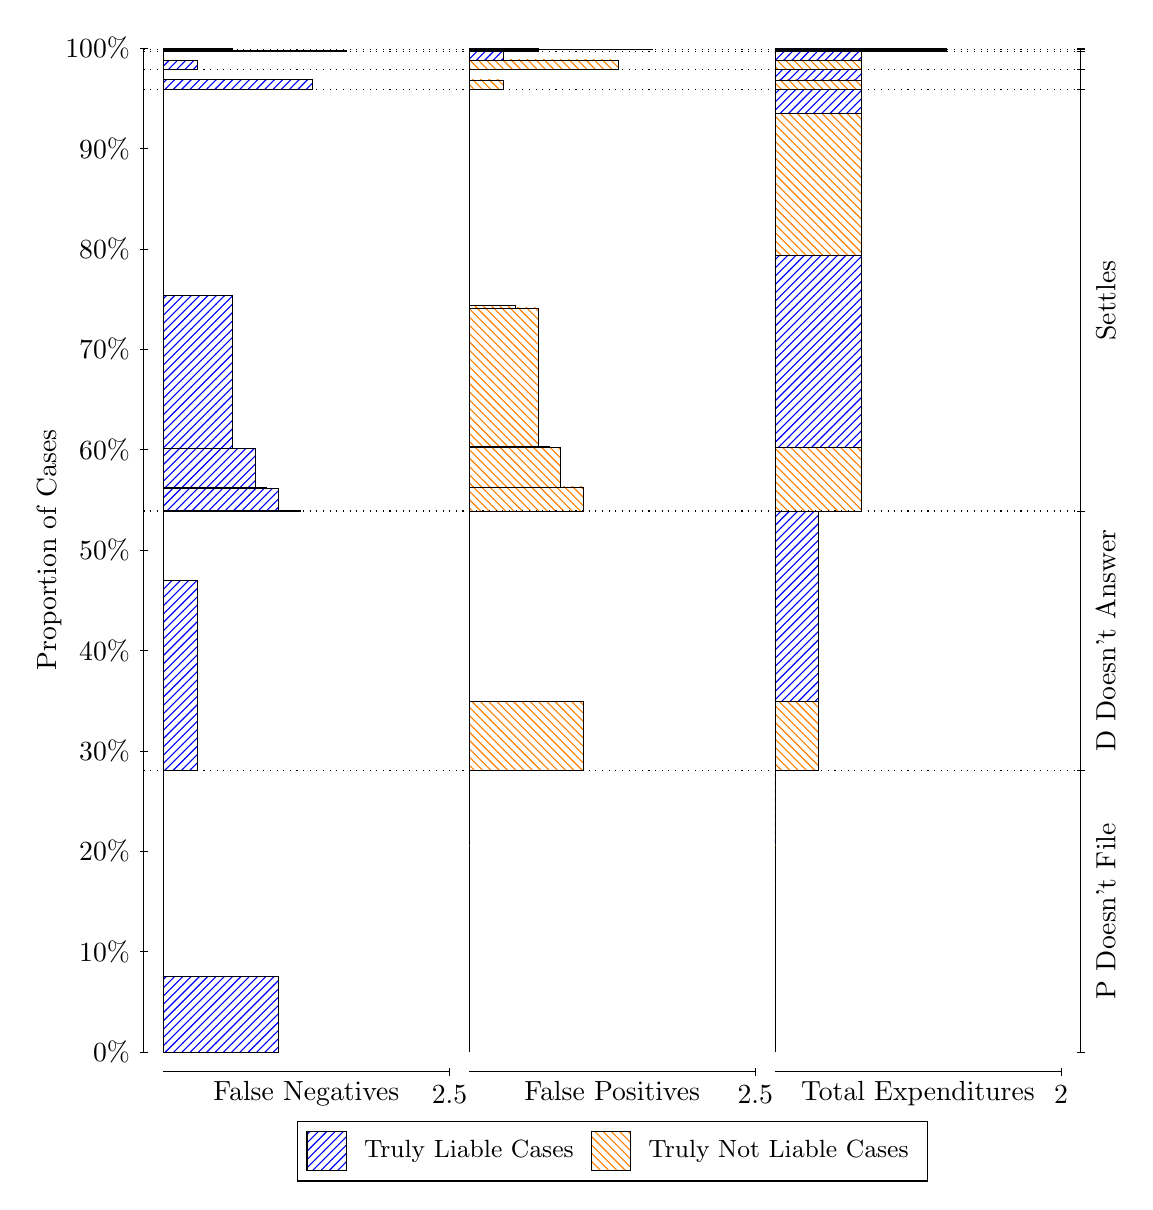
\begin{tikzpicture}
\draw[black, very thin] (1.5,1.75) -- (1.5,14.5);
\node[rotate=90, text=black, anchor=center] at (0.3, 8.125) {Proportion of Cases};
\draw[black, very thin] (1.45,1.75) -- (1.55,1.75);
\node[text=black, anchor=east] at (1.45, 1.75) {0\%};
\draw[black, very thin] (1.45,3.025) -- (1.55,3.025);
\node[text=black, anchor=east] at (1.45, 3.025) {10\%};
\draw[black, very thin] (1.45,4.3) -- (1.55,4.3);
\node[text=black, anchor=east] at (1.45, 4.3) {20\%};
\draw[black, very thin] (1.45,5.575) -- (1.55,5.575);
\node[text=black, anchor=east] at (1.45, 5.575) {30\%};
\draw[black, very thin] (1.45,6.85) -- (1.55,6.85);
\node[text=black, anchor=east] at (1.45, 6.85) {40\%};
\draw[black, very thin] (1.45,8.125) -- (1.55,8.125);
\node[text=black, anchor=east] at (1.45, 8.125) {50\%};
\draw[black, very thin] (1.45,9.4) -- (1.55,9.4);
\node[text=black, anchor=east] at (1.45, 9.4) {60\%};
\draw[black, very thin] (1.45,10.675) -- (1.55,10.675);
\node[text=black, anchor=east] at (1.45, 10.675) {70\%};
\draw[black, very thin] (1.45,11.95) -- (1.55,11.95);
\node[text=black, anchor=east] at (1.45, 11.95) {80\%};
\draw[black, very thin] (1.45,13.225) -- (1.55,13.225);
\node[text=black, anchor=east] at (1.45, 13.225) {90\%};
\draw[black, very thin] (1.45,14.5) -- (1.55,14.5);
\node[text=black, anchor=east] at (1.45, 14.5) {100\%};

\draw[black, very thin] (13.4,1.75) -- (13.4,14.5);
\draw[black, very thin] (13.35,1.75) -- (13.45,1.75);
\node[anchor=west] at (13.35, 1.75) {};
\draw[black, very thin] (13.35,5.3259) -- (13.45,5.3259);
\node[anchor=west] at (13.35, 5.3259) {};
\draw[black, very thin] (13.35,8.6203) -- (13.45,8.6203);
\node[anchor=west] at (13.35, 8.6203) {};
\draw[black, very thin] (13.35,13.97) -- (13.45,13.97);
\node[anchor=west] at (13.35, 13.97) {};
\draw[black, very thin] (13.35,14.23) -- (13.45,14.23);
\node[anchor=west] at (13.35, 14.23) {};
\draw[black, very thin] (13.35,14.46) -- (13.45,14.46);
\node[anchor=west] at (13.35, 14.46) {};
\draw[black, very thin] (13.35,14.48) -- (13.45,14.48);
\node[anchor=west] at (13.35, 14.48) {};
\draw[black, very thin] (13.35,14.5) -- (13.45,14.5);
\node[anchor=west] at (13.35, 14.5) {};

\draw[black, very thin, pattern color=blue, pattern=north east lines] (1.75,1.75) rectangle (3.2033,2.7051);
\draw[black, very thin, pattern color=orange, pattern=north west lines] (1.75,2.7051) rectangle (1.75,5.3259);
\draw[black, very thin, pattern color=blue, pattern=north east lines] (1.75,5.3259) rectangle (2.186,7.7435);
\draw[black, very thin, pattern color=orange, pattern=north west lines] (1.75,7.7435) rectangle (1.75,8.6203);
\draw[black, very thin, pattern color=blue, pattern=north east lines] (1.75,8.6203) rectangle (3.494,8.6293);
\draw[black, very thin, pattern color=blue, pattern=north east lines] (1.75,8.6293) rectangle (3.2033,8.9109);
\draw[black, very thin, pattern color=blue, pattern=north east lines] (1.75,8.9109) rectangle (3.058,8.9191);
\draw[black, very thin, pattern color=blue, pattern=north east lines] (1.75,8.9191) rectangle (2.9127,9.4161);
\draw[black, very thin, pattern color=blue, pattern=north east lines] (1.75,9.4161) rectangle (2.622,11.357);
\draw[black, very thin, pattern color=orange, pattern=north west lines] (1.75,11.357) rectangle (1.75,13.97);
\draw[black, very thin, pattern color=blue, pattern=north east lines] (1.75,13.97) rectangle (3.6393,14.105);
\draw[black, very thin, pattern color=orange, pattern=north west lines] (1.75,14.105) rectangle (1.75,14.23);
\draw[black, very thin, pattern color=blue, pattern=north east lines] (1.75,14.23) rectangle (2.186,14.341);
\draw[black, very thin, pattern color=orange, pattern=north west lines] (1.75,14.341) rectangle (1.75,14.46);
\draw[black, very thin, pattern color=blue, pattern=north east lines] (1.75,14.46) rectangle (4.0753,14.466);
\draw[black, very thin, pattern color=orange, pattern=north west lines] (1.75,14.466) rectangle (1.75,14.48);
\draw[black, very thin, pattern color=blue, pattern=north east lines] (1.75,14.48) rectangle (2.622,14.494);
\draw[black, very thin, pattern color=orange, pattern=north west lines] (1.75,14.494) rectangle (1.75,14.5);
\draw[black, very thin, pattern color=orange, pattern=north west lines] (5.6333,1.75) rectangle (5.6333,4.3708);
\draw[black, very thin, pattern color=blue, pattern=north east lines] (5.6333,4.3708) rectangle (5.6333,5.3259);
\draw[black, very thin, pattern color=orange, pattern=north west lines] (5.6333,5.3259) rectangle (7.0867,6.2027);
\draw[black, very thin, pattern color=blue, pattern=north east lines] (5.6333,6.2027) rectangle (5.6333,8.6203);
\draw[black, very thin, pattern color=orange, pattern=north west lines] (5.6333,8.6203) rectangle (7.0867,8.9269);
\draw[black, very thin, pattern color=orange, pattern=north west lines] (5.6333,8.9269) rectangle (6.796,9.425);
\draw[black, very thin, pattern color=orange, pattern=north west lines] (5.6333,9.425) rectangle (6.6507,9.4413);
\draw[black, very thin, pattern color=orange, pattern=north west lines] (5.6333,9.4413) rectangle (6.5053,11.201);
\draw[black, very thin, pattern color=orange, pattern=north west lines] (5.6333,11.201) rectangle (6.2147,11.234);
\draw[black, very thin, pattern color=blue, pattern=north east lines] (5.6333,11.234) rectangle (5.6333,13.97);
\draw[black, very thin, pattern color=orange, pattern=north west lines] (5.6333,13.97) rectangle (6.0693,14.096);
\draw[black, very thin, pattern color=blue, pattern=north east lines] (5.6333,14.096) rectangle (5.6333,14.23);
\draw[black, very thin, pattern color=orange, pattern=north west lines] (5.6333,14.23) rectangle (7.5227,14.349);
\draw[black, very thin, pattern color=blue, pattern=north east lines] (5.6333,14.349) rectangle (6.0693,14.46);
\draw[black, very thin, pattern color=orange, pattern=north west lines] (5.6333,14.46) rectangle (6.5053,14.473);
\draw[black, very thin, pattern color=blue, pattern=north east lines] (5.6333,14.473) rectangle (5.6333,14.48);
\draw[black, very thin, pattern color=orange, pattern=north west lines] (5.6333,14.48) rectangle (7.9587,14.486);
\draw[black, very thin, pattern color=blue, pattern=north east lines] (5.6333,14.486) rectangle (6.5053,14.5);
\draw[black, very thin, pattern color=orange, pattern=north west lines] (9.5167,1.75) rectangle (9.5167,4.3708);
\draw[black, very thin, pattern color=blue, pattern=north east lines] (9.5167,4.3708) rectangle (9.5167,5.3259);
\draw[black, very thin, pattern color=orange, pattern=north west lines] (9.5167,5.3259) rectangle (10.062,6.2027);
\draw[black, very thin, pattern color=blue, pattern=north east lines] (9.5167,6.2027) rectangle (10.062,8.6203);
\draw[black, very thin, pattern color=orange, pattern=north west lines] (9.5167,8.6203) rectangle (10.607,9.425);
\draw[black, very thin, pattern color=blue, pattern=north east lines] (9.5167,9.425) rectangle (10.607,11.862);
\draw[black, very thin, pattern color=orange, pattern=north west lines] (9.5167,11.862) rectangle (10.607,13.671);
\draw[black, very thin, pattern color=blue, pattern=north east lines] (9.5167,13.671) rectangle (10.607,13.97);
\draw[black, very thin, pattern color=orange, pattern=north west lines] (9.5167,13.97) rectangle (10.607,14.096);
\draw[black, very thin, pattern color=blue, pattern=north east lines] (9.5167,14.096) rectangle (10.607,14.23);
\draw[black, very thin, pattern color=orange, pattern=north west lines] (9.5167,14.23) rectangle (10.607,14.349);
\draw[black, very thin, pattern color=blue, pattern=north east lines] (9.5167,14.349) rectangle (10.607,14.46);
\draw[black, very thin, pattern color=orange, pattern=north west lines] (9.5167,14.46) rectangle (11.697,14.473);
\draw[black, very thin, pattern color=blue, pattern=north east lines] (9.5167,14.473) rectangle (11.697,14.48);
\draw[black, very thin, pattern color=orange, pattern=north west lines] (9.5167,14.48) rectangle (11.697,14.486);
\draw[black, very thin, pattern color=blue, pattern=north east lines] (9.5167,14.486) rectangle (11.697,14.5);
\draw[black, dotted] (1.5,5.3259) -- (13.4,5.3259);
\draw[black, dotted] (1.5,8.6203) -- (13.4,8.6203);
\draw[black, dotted] (1.5,13.97) -- (13.4,13.97);
\draw[black, dotted] (1.5,14.23) -- (13.4,14.23);
\draw[black, dotted] (1.5,14.46) -- (13.4,14.46);
\draw[black, dotted] (1.5,14.48) -- (13.4,14.48);
\draw[black, very thin] (1.75,1.5) -- (5.3833,1.5);
\node[text=black, anchor=north] at (3.5667, 1.5) {False Negatives};
\draw[black, very thin] (5.3833,1.45) -- (5.3833,1.55);
\node[text=black, anchor=north] at (5.3833, 1.45) {2.5};

\draw[black, very thin] (5.6333,1.5) -- (9.2667,1.5);
\node[text=black, anchor=north] at (7.45, 1.5) {False Positives};
\draw[black, very thin] (9.2667,1.45) -- (9.2667,1.55);
\node[text=black, anchor=north] at (9.2667, 1.45) {2.5};

\draw[black, very thin] (9.5167,1.5) -- (13.15,1.5);
\node[text=black, anchor=north] at (11.333, 1.5) {Total Expenditures};
\draw[black, very thin] (13.15,1.45) -- (13.15,1.55);
\node[text=black, anchor=north] at (13.15, 1.45) {2};

\node[text=black, centered, rotate=90] at (13.72, 3.538) {P Doesn't File};
\node[text=black, centered, rotate=90] at (13.72, 6.9731) {D Doesn't Answer};
\node[text=black, centered, rotate=90] at (13.72, 11.295) {Settles};





\draw (7.449999999999999,1.5) node[draw=none] (baseCoordinate) {};
\begin{scope}[align=center]
        \matrix[scale=0.5, draw=black, below=0.5cm of baseCoordinate, nodes={draw}, column sep=0.1cm]{
            \node[rectangle, draw, minimum width=0.5cm, minimum height=0.5cm, pattern color=blue, pattern=north east lines] {}; &
            \node[draw=none, font=\small, text=black] (B) {Truly Liable Cases}; &
            \node[rectangle, draw, minimum width=0.5cm, minimum height=0.5cm, pattern color=orange, pattern=north west lines] {}; &
            \node[draw=none, font=\small, text=black] (B) {Truly Not Liable Cases}; \\
            };
\end{scope}

\end{tikzpicture}
\end{document}